% \documentclass{template/socthesis}
\documentclass[12pt, a4paper]{article}

\usepackage[utf8]{inputenc}
\usepackage[czech,shorthands=off]{babel}

% \usepackage[T1]{fontenc} % výstupní kódování
\usepackage{subcaption}
\usepackage{amsmath}
\usepackage{enumitem}
\usepackage{hyperref} % reference
\usepackage{gensymb} % balíček symbolů
\usepackage{booktabs}

\usepackage[toc,page]{appendix}
\usepackage{color} % balíček pro obarvování textů
\usepackage{xcolor}  % zapne možnost používání barev, mj. pro \definecolor
\definecolor{mygreen}{RGB}{0,150,0} % nastavení barev odkazů
\usepackage{listings} % balíček pro formátování zdrojových kódů
\usepackage{multirow}
\usepackage{pifont}
\usepackage{pdfpages}
\usepackage{parskip}
\usepackage[margin=25mm]{geometry}
\usepackage[backend=bibtex]{biblatex}
\usepackage[author=,status=draft]{fixme} % vkládání poznámek
% dva módy (status): draft (poznámky se zobrazují v PDF) / final (poznámky se nezobrazují v PDF)



\newcommand{\cmark}{\textcolor{green}{\ding{51}}}%
\newcommand{\xmark}{\textcolor{red}{\ding{55}}}%

\lstset { %
    language=C++,
    backgroundcolor=\color{black!5}, % set backgroundcolor
    basicstyle=\footnotesize,% basic font setting
}

\setlist[itemize]{parsep=1pt}

\addbibresource{text.bib} % soubor s bibliografií
% \nocite{*}


% hinty k používání balíčků hyperref, url, hyperlink a hypertarget
% \usepackage{hyperref} % balíček pro hypertextové odkazy
% \url{www.odkaz.cz}
% \href{http://www.odkaz.cz}{Text který bude jako odkaz}
% \hyperlink{label}{proklikávací_text} - odkaz na text
% \hypertarget{label}{cíl_odkazu} - cíl odkazu
\title{Integration into Industry 4.0}
\author{Jakub Andrýsek}
\date{}

\begin{document} % konec preambule dokumentu

\maketitle

% #########################################################################################
\section*{Abstract}
I designed a production monitoring system that can record measured data and submit them from machines to a server via the wireless network in real-time.



% #########################################################################################
\section*{Introduction}

CZ

Práce s názvem Integrace do průmyslu 4.0 se zabývá návrhem monitorovacího systému pro výrobní stroje a jeho nasazením ve firmě ROTEX Vysočina s.r.o.
Tato firma se věnuje výrobě ponožek.
Pracuje ve dvousměnném provozu a produkuje měsíčně přes dvanáct tisíc párů ponožek.

Ve firmě je 25 pletacích strojů na ponožky, o které se v každé směně starají tři operátoři.
Samotná práce operátora spočívá v kontrole upletených ponožek, otáčení dopletených ponožek a opravách porouchaných strojů.

Systém je interně pojmenován iSocks IoT.
Jeho úkolem je monitoring počtu upletených ponožek, zaznamenávání doby zastavení jednotlivých strojů, porovnávání jednotlivých směn, ale také podání přehledu zaměstnavateli o aktuální produkci.

Dříve firma neměla žádná data o době pletení, denní  produkci, nebo čase zapnutí strojů.
To vše  můj systém řeší  a nabízí jednoduché, uživatelsky přívětivé rozhraní, kde si uživatel všechny tyto údaje přehledně zobrazí v grafech a v tabulkách.

EN

This project with the name Integration into Industry 4.0 deals with the design of a monitoring system for production machines and its deployment in ROTEX Vysočina s.r.o.
This company is engaged in the production of socks.
It operates in two-dimensional production and produces monthly over a hundred and twenty-five thousand pairs of socks.

In the company, there are 25 sock knitting machines, which are operated by three operators.
The whole work of the operator consists of checking finished socks and fixing the machines.

The system is internally called iSocks IoT.
The goal of the system is to monitor the number of finished socks, measure time when the machine is in error state, and compare the different phases, but also to provide a summary to the employees about the current production.
% The system is designed to be easy to use, and to be easy to understand.

In the past, the company had no data about the time of knitting machines, the daily production, or the time of starting the machines.
My system solves this problem and provides an easy, user-friendly interface, where the user can easily see all these data in graphs and tables.

\newpage

\begin{figure}[t]
    \centering
    \includegraphics[width=0.7\textwidth]{img/V2-uchyceni.png}
    \caption{Senzor na stroji}
    \label{fig:SenzorNaStroji}
\end{figure}


% #########################################################################################
\section*{Aims}
CZ

Tato práce představuje ucelený systém pro automatický monitoring průmyslové výroby a jeho nasazení do praxe.
Systém byl navrhován jako univerzální platforma pro monitoring výrobních strojů, s primárním zaměřením na pletací stroje.

Cílem této práce bylo navrhnout ucelený systém, který dokáže:

\begin{itemize}
    \item automaticky počítat upletené ponožky
    \item on-line hlásit poruchu na stroji a zjišťovat celkovou poruchovost strojů
    \item porovnávat výkonnost jednotlivých pracovních směn
    \item monitorovat průběh výroby
    \item nahradit část monotónní práce operátora
    \item zrychlit a zefektivnit výrobu
    \item snížit chybovost
\end{itemize}

EN

This project aims to design a system for automatic monitoring of production machines and their deployment into practice.
The system was designed as a universal platform for monitoring production machines, with the primary focus on sock knitting machines.

The goal of this project was to design a system that:

\begin{itemize}
    \item automatically counts finished socks
    \item online reports machine failures and determines the total failure rate of the machines
    \item compares the efficiency of each working phase
    \item monitors the production process
    \item replaces the part of monotonous work of the operator
    \item speeds up and effectively improves the production
    \item reduces the error rate
\end{itemize}


% #########################################################################################
\section*{Materials and methods}
CZ

Systém se skládá ze senzorové části, serveru a podpůrného serveru.
Senzorová část je postavená na vlastní senzorové desce s mikrokontrolérem s barevným displejem.
Senzor je připojen k pletacímu stroji a odesílá naměřená data.
Server přijímá  data ze senzorů, zajišťuje jejich zpracování a následné zobrazení uživateli.
Podpůrný server se stará o aktualizaci a o kontrolu správného chodu senzorů.

Systém byl navrhován jako univerzální platforma pro monitoring výrobních strojů s primárním zaměřením na pletací stroje.
Samotné nasazení tohoto systému proběhlo ve firmě ROTEX Vysočina s.r.o. zaměřující se na pletení ponožek.
Ve firmě jsem nasadil senzory na 10 pletacích strojů, které zde běží již 18 měsíců.
Za tuto dobu systém zaznamenal přes XXX upletených ponožek.
Tento systém ve firmě ROTEX monitoruje počet upletených ponožek, dobu stání jednotlivých strojů, ale také porovnává jednotlivé pracovní směny.

EN

The system consists of a sensor part, a server, and a supporting server.
The sensor part is built on a circuit board with a microcontroller.
The sensor is connected to the sock knitting machine and sends measured data to the server.
The server receives data from the sensors, processes them, and displays them to the user.
The supporting server is responsible for updating and checking the correct operation of the sensors.

The system was designed as a universal platform for monitoring production machines with a primary focus on sock knitting machines.
The actual deployment of this system took place in the company ROTEX Vysočina s.r.o. focused on the production of socks.
I deployed my system on ten sock knitting machines, which were operating for 18 months.
During this time the system recorded over XXX finished socks.
This system in the company ROTEX monitors the number of finished socks, the time it takes to stop each machine, and compares the different phases, but also provides a summary to the employees about the current production.


% #########################################################################################
\subsection*{Sensors}
CZ

Pletací stroje na ponožky jsou starší zařízení bez podpory připojení k internetu.
Pro měření jsem tedy musel vyvinout vlastní  senzory, které získávají data z elektrických součástek na pletacích  strojích a skrze WiFi připojení je posílají  na server.
Senzory iSocks IoT jsem navrhoval tak, aby se daly jednoduše připojit na stávající pletací stroje a napojit je tak do centrálního řídícího systému.
Dalším požadavkem senzoru bylo, aby neohrožoval chod samotného stroje, pokud není můj systém aktivní, nemá to žádný vliv na zbylý chod firmy.

Senzory jsou postavené na mikrokontroléru ESP32, který nabízí dostatečný výkon a má bezdrátovou konektivitu WiFi.
Každý z těchto senzorů má svoje jedinečné číslo, pod kterým posílá naměřená data na server.
Senzor je napájen z 5 nebo 24 V a má spotřebu 120 mA (on 5 V).

EN

The socks machines are old machines without support for internet connection and remote monitoring.
For measuring, I had to develop my sensors, which get data from electrical components on sock knitting machines and send them to the server via WiFi connection.
Sensors iSocks IoT were designed to be easily connected to existing sock knitting machines and to connect them to the central control system.
Another requirement of the sensor was to prevent damage to the machine if it was not active, it does not affect the remaining operation of the company.

Sensors are built on an ESP32 microcontroller, which provides enough performance and WiFi connectivity.
Each of those sensors has its unique number, under which it sends the measured data to the server.
The sensor is powered from 5 or 24 V and has a consumption of 120 mA (on 5 V).

\begin{figure}[t]
    \centering
    \includegraphics[width=0.7\textwidth]{img/oba.png}
    \caption{Sensors: first version on the left, second version on the right}
    \label{fig:dveVerze}
\end{figure}

CZ

Na každém senzoru jsou dva optočleny napojené na indikační diody pletacího stroje.
Z jedné diody se snímá zastavení stroje pro výpočet poruchového času a z druhé senzor získává počet upletených ponožek.
Na těchto dvou údajích je postavený celý měřící a výpočetní systém.
Dále senzor obsahuje dvě uživatelská tlačítka sloužící pro nastavení jedinečného ID senzoru.
Pro rychlé grafické znázornění jsou na desce také dvě barevné diody.

Hlavní vizuální roli zajišťuje LCD displej, na kterém se operátorům zobrazují základní údaje o stroji.
Ve vrchní části jsou vypsány údaje o bezdrátovém připojení a číslo senzoru.
Uprostřed se operátorovi velkým písmem zobrazuje počet upletených ponožek a v případně zastavení stroje čas odstávky.
Tyto údaje se na každém stroji výrazně vykreslují a upozorňují tak obsluhu k brzké opravě.
Poslední novinku, kterou jsem na senzory doprogramoval je zobrazování průměrné rychlosti pletení ponožek za hodinu.
S takovýmto typem rychlosti se každodenně setkáváme například v autě a operátor z ní dokáže rychle dopočítat čas dopletení zakázky.

Pro upevnění senzoru jsem vytvořil kompaktní 3D tištěnou krabičku.
Tu jsem navrhoval v programu Fusion 360 a následně jsem ji vytiskl na 3D tiskárně.

EN

There are two optocouplers on each sensor connected to state indicator LEDs on the sock knitting machine.
One of those LED is used to measure the time it takes to stop the machine for a breakdown and the second diode is used to determine the number of finished socks.
On those two LEDs is built the whole measuring and counting system.
Additionally, the sensor has two user buttons used to set a unique ID of the sensor.
There are two colored LEDs for direct state indication on the board.

The main information can operator saw on the integrated LCD.
On the top of the display is displayed the connection status and the number of finished socks.
The operator can see the number of finished socks and the time of repairing the machine.
This information is displayed on each machine and helps to fix the machine quickly.
The last new feature that I added to the sensor is the display of the average speed of knitting per hour.
This average speed is displayed on each machine and is used to calculate the time it takes to finish a knitting order.

The sensor is mounted to the compact 3D printed box.
It was designed in Fusion 360 and printed on the FDM 3D printer.

% #########################################################################################
\subsection*{Web server}

CZ

Nedílnou součástí tohoto systému je také serverová část, která se stará o přijímání naměřených dat, jejich zpracování a následné zobrazení uživateli.
Samotný server běží na mikropočítači Raspberry Pi 4 Modelu B.

Na zařízení běží operační systém Raspberry Pi OS s grafickým rozhraním.
Webové stránky běží na HTTP serveru Apache2 a PHP 8.0.
Jako databázový systém využívám MariaDB.
Server běží lokálně uvnitř firmy v zabezpečené síti, díky čemuž je systém rychlý a nezávislý na internetovém připojení.

Na webový server se dá jednoduše připojit otevřením lokálního firemního odkazu \newline\href{http://pletacka.local}{pletacka.local}.
Poté se uživateli zobrazí úvodní přehledová stránka s barevnými bublinami, které představují jednotlivé pletací stroje.
Jejich barva pak udává v jakém stavu se stroj aktuálně nachází. Uživatel tak dokáže velmi rychle zjistit aktuální funkčnost pletacích strojů bez nutnosti návštěvy pletárny.
Kromě barvy se v bublině zobrazuje také text, ten ukazuje počet upletených ponožek a v případě zastavení stroje a zčervenání se text změní na dobu zastavení stroje.

EN

The second part of this system is the web server part, which receives the measured data, processes it, and then displays it to the user.
The web server runs on a Raspberry Pi 4 Model B.

The server is running on a Raspberry Pi OS with a graphical interface.
The web pages are running on Apache2 and PHP 8.0.
As a system database, I use MariaDB.

The server is running locally inside the company network, which makes it fast and independent from the internet connection.

To connect to the web server you can open a local company link \newline\href{http://iSocks.local}{iSocks.local}.
Then you will see the welcome page with colored bubbles that represent the knitting machines.
The color of the bubble shows the current state of the machine.
You can quickly determine the current state of the knitting machines without having to visit the knitting factory.
Besides the color of the bubble, there is also a text that shows the number of finished socks and the time it takes to stop the machine for a breakdown.


\begin{figure}[t]
    \centering
    \includegraphics[width=0.9\textwidth]{img/Uvod.png}
    \caption{Home page}
    \label{fig:webUvod}
\end{figure}

CZ

Další webovou stránkou jsou Přehledy ze senzorů generované pro každý pletací stroj.
Zde se uživateli zobrazují data v různých časových přehledech.
Pro snadné porovnání dat mezi dvěma směnami se tyto údaje zobrazují vedle sebe.
Pod číselnými přehledy jsou pak předgenerované dlouhodobé grafy viz \ref{fig:webSenzory}

Každý senzor využívá pět databázových tabulek. První slouží k ukládání surových dat, do zbylých tabulek se pak ukládají automaticky generované přehledy.
Ty slouží k rychlému vykreslení grafů a výpočtu dlouhodobých údajů.
Senzor zaznamená dopletenou ponožku a skrze REST API posílá naměřený údaj na webový server, ten ji zkontroluje a uloží do databáze ke konkrétnímu senzoru.
Každý databázový záznam obsahuje číslo stroje, unikátní ID události, naměřený stav a čas události.

EN

The next web pages are the summaries of the sensors generated for each knitting machine.
Here the user can see the data in different time summaries.
For easy comparison between two work shifts, these data are displayed beside each other.
At the end of the summaries are generated long-term graphs viz \ref{fig:webSenzory}

Each sensor uses five database tables. The first one is used to store raw data, the other ones are automatically generated summaries.
These summaries are used to quickly draw graphs and calculate long-term data.
The sensor records the finished sock and sends the data to the web server, which checks it and saves it to the database for the specific sensor.
Each database entry contains the number of the machine, a unique ID of the event, the measured state, and the time of the event.

% \includepdf[pages=-, scale=0.6, pagecommand={}]{DATASHEET/Pletacka_board_v2.pdf}
\begin{figure}[htbp]
    \centering
    % \includegraphics[scale=0.5]{DATASHEET/Pletacka_board_v2.pdf}
    \includegraphics[width=\textwidth]{DATASHEET/Pletacka_board_v2.pdf}
    \caption{Schematic of the sensor}
    \label{fig:Schemav1}
\end{figure}


\begin{figure}[t]
    \centering
    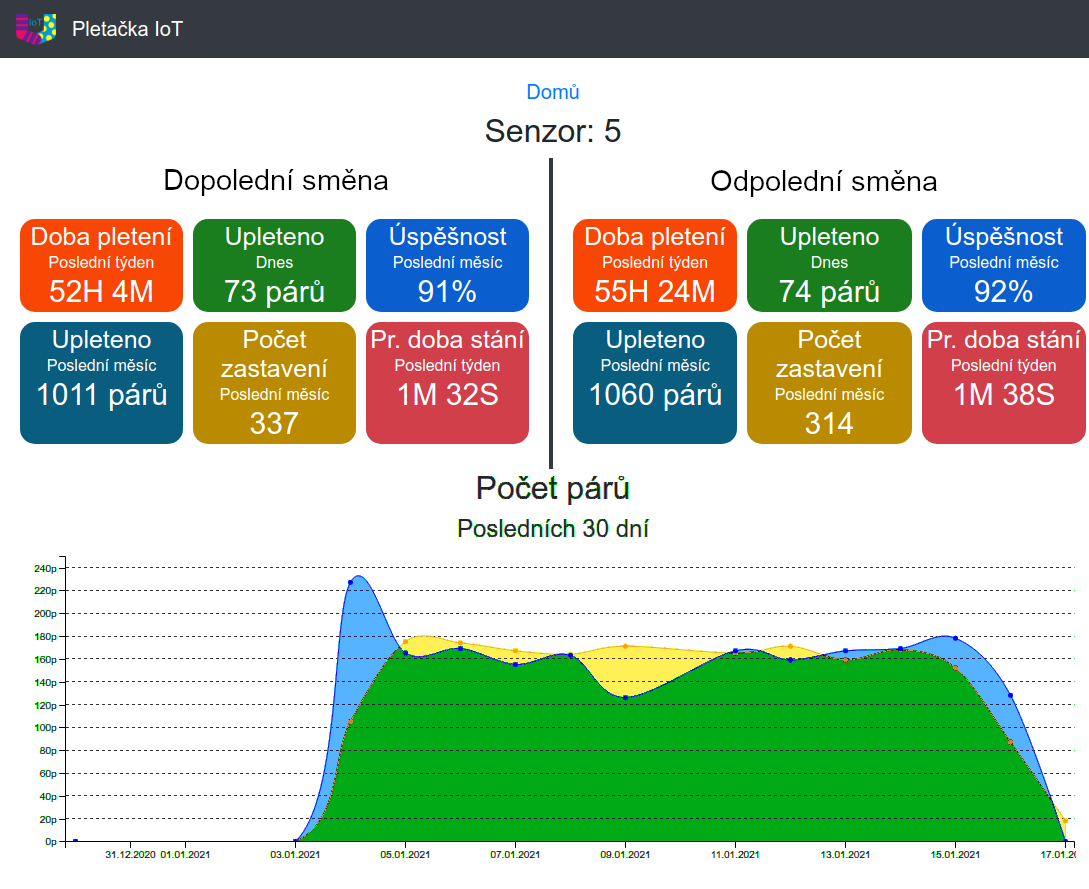
\includegraphics[width=0.7\textwidth]{img/prehled.png}
    \caption{Sensor charts}
    \label{fig:webSenzory}
\end{figure}


% #########################################################################################
\subsection*{Support server}

CZ

Podpůrný server vznikl jako rozšíření pro senzory.
Server je naprogramovaný v Pythonu a běží na Raspberry Pi společně s webovým serverem.\newline

Hlavním úkolem tohoto serveru je detekce zapnutých senzorů.
Na serveru běží takzvaný Watchdog.
Jde o periodickou smyčku, která každé čtyři vteřiny čeká na zprávu ze senzoru.
Touto zprávou se senzor nahlásí, že je zapnutý. Pokud takováto zpráva nedojde do deseti vteřin, je senzor prohlášen za vypnutý a v databázi se označí jako neaktivní.

EN

The support server was created as an extension for sensors.
The server is programmed in Python and runs on Raspberry Pi together with the web server.\newline

The main task of this server is the detection of turned-on sensors.
On the server, there is a Watchdog.
This is a periodic loop that waits for a message from the sensor.
This message is used to signal that the sensor is turned on.
If such a message does not arrive in ten minutes, the sensor is marked as turned off and in the database, it is marked as inactive.


% #########################################################################################
\subsection*{Princip fungování iSocks IoT}

CZ

V předchozích kapitolách byly popsány části systému iSocks IoT.
V této kapitole bude celý systém popsán jako celek.

První, a zároveň nejdůležitější částí, je získávání dat pomocí senzorů.
Jakmile senzor zaznamená jakoukoliv změnu, okamžitě tuto zprávu odesílá na server.
Odesílání probíhá skrze senzorové API, kde se nejdříve senzor ověří a následně se stav zapíše do databáze k příslušnému senzoru.
Po zapsání do databáze se vrátí do senzoru zpráva o provedení zápisu.

Dalším krokem je zpracovávání surových dat z databáze.
K tomuto účelu běží na serveru výběrové API, které je automaticky spouštěné v nastavený čas.
Slouží ke generování širších výběrů dat, hodinové, denní, měsíční a roční výběry.
Tyto výběry se následně ukládají do databáze k danému senzoru.
Generování těchto dat probíhá převážně v noci, kdy je server nejméně vytížen.

Posledním krokem je zobrazení dat uživateli.
Je to jediná část, se kterou se běžný uživatel dostane do kontaktu.
Proto je nutné, aby zobrazení bylo co nejrychlejší a pro uživatele co nejpříjemnější.
K rychlému zobrazování se využívají před generované výběry, ke kterým se dopočítají dosud nezpracovaná data a celý výsledek se zobrazí uživateli.

EN

In previous chapters were described parts of the iSocks IoT system.
In this chapter, the whole system will be described as a single unit.

The first and most important part of the system is data acquisition.
Once the sensor detects any change, it immediately sends the message to the server.
The message is sent through the sensor API, where the sensor is first verified and then the state is written to the database for the specific sensor.
After writing to the database the message is returned from the sensor.

The next step is the processing of raw data from the database.
This is done on the server by the acquisition API, which is automatically started at the specified time.
These selections are used to generate longer selections, hourly, daily, monthly, and yearly.
These selections are then stored in the database for the specific sensor.
Generation of these data is done mostly at night when the server is least busy.

The last step is displaying data to the user.
This is the only part that the user receives in contact with the system.
So it is necessary that the display is as quick as possible and that the user is as pleasant as possible.
For a quick display, the selections that have been generated are used, together with the data that has not yet been processed and the result is displayed to the user.

EN2

In previous chapters were described parts of the iSocks IoT system.
In this chapter, the whole system will be described as a single unit.

The first and most important part of the system is the acquisition of data using sensors.
Once the sensor detects any change, it immediately sends the message to the server.
The transmission of this message is performed by the sensor API, where first the sensor is checked and then the state is written to the database for the specific sensor.
After writing to the database the server returns a message about the writing.

The second step is the processing of raw data from the database.
This is performed on the server API, which is automatically started at the specified time.
This is used to generate longer time summaries, hours, days, months, and years.
These summaries are then saved to the database for the specific sensor.
The generation of these data is performed mostly at night when the server is least busy.

The last step is displaying data to the user.
This is the only part of the system that the user receives to contact.
So it is necessary to make the display as fast as possible and to make it as pleasant for the user.
For fast display of the result of the calculations, the generated summaries are used, which are generated before the calculations and which are used to display the result to the user.

EN3 JPA

In previous chapters were described parts of the iSocks IoT system.
In this chapter, the whole system will be described as a single unit.

The first and most important part of the system is the acquisition of data using sensors.
Once the sensor detects any change, it immediately sends the message to the server.
The transmission of this message is performed by the sensor API, where first the sensor is checked and then the state is written to the database for the specific sensor.
After writing to the database the server returns a confirmation message.

The second step is the processing of raw data from the database.
This is performed on the server API, which is automatically started at the specified time.
This is used to generate longer time summaries, hours, days, months, and years.
These summaries are then saved to the database for the specific sensor.
The generation of these data is performed mostly at night when the server is least busy.

The last step is displaying data to the user.
This is the only part of the system that normal user is going to see and control.
So it is necessary to make the display as fast as possible and to make it as pleasant for the user.
For fast display of the result of the calculations, the generated summaries are used, which are generated before the calculations and which are used to display the result to the user.


\begin{figure}[t]
    \centering
    \includegraphics[width=0.9\textwidth]{img/Princip.png}
    \caption{Data processing}
    \label{fig:princip}
\end{figure}


% #########################################################################################
\subsection*{Testing}

CZ

Celý systém jsem vyvíjel od února 2020.
První malé testy probíhaly již od května 2020, ale k většímu nasazení došlo až v září a listopadu 2020.
Od té doby je systém ve firmě nasazen a průběžně probíhá kontrola měření a funkčnosti.

EN
I have been developing the entire system since February 2020.
The first small tests were performed in May 2020, but the full system was tested in the summer of 2020 and in the Autumn of 2020.
From then on the system is tested and maintained in the company.


% #########################################################################################
\newpage
\section*{Results and discussion}

CZ

Cíle této práce byly splněny. Ze starých, ale výrobně funkčních stojů, se díky mému systému staly moderní online stroje.
Systém zefektivnil výrobu, šetří čas operátora, nahrazuje rutinní úkony vykonávané doposud operátorem a přináší detailní přehled o výrobě včetně vzájemného porovnání výrobních směn.
System iSocks IoT tak snižuje výrobní náklady při výrobě a to jednak v podobě minimalizace prostojů stroje při poruše, tak ušetřením času operátora při výrobě.


Všechny tyto vytyčené cíle se mi podařilo splnit.
Systém nadále běží ve firmě ROTEX Vysočina s.r.o a pomáhá v běžném provozu.
Můj systém se stal nedílnou součástí výrobního procesu a analyzuje a zefektivňuje průběh výroby.

Systém je k 20. červnu 2021 nasazen na deseti pletacích strojích a po dobu provozu zaznamenal již přes sto padesát tisíc upletených ponožek bez závady na senzorech.

Velkým přínosem pro firmu je porovnávání pracovních směn, díky kterým zaměstnavatel ihned vidí rozdíly mezi produktivitou práce v daném čase.

Díky této práci jsem se naučil navrhovat plošné spoje, rozšířil jsem si obzory v elektronice a při vývoji jsem si vyzkoušel práci s měřícími přístroji.
Také jsem se naučil programovat v jazyce PHP a vytvářet komplexní webové systémy.

V budoucnu bych chtěl tento systém rozšířit na všechny pletací stroje a pokrýt tak celou výrobu.
Taktéž pokračuji na vylepšování webové aplikace a plánuji ji rozšířit o další funkce, například o export dat do tabulek.

Všechny zdrojové kódy a DPS k projektu jsou k dispozici na \url{https://github.com/Pletacka-IoT} pod MIT licencí.

EN

All the goals of the project set at the beginning were achieved. From the simple old system, it developed to the modern online system.
The system improved production time, reduced operator time and introduced a detailed overview of the product including a comparison of changes in production.
The system reduced the production cost by minimizing the manufacturing time.


All these objectives were met.
The system is currently used in ROTEX Vysočina s.r.o. The system is part of the production process. It analyzes and improves production.

As of June 20, 2021, the system is deployed on ten knitting machines and has already recorded over one hundred and fifty thousand knitted socks without a sensor malfunction.

A big advantage of this system is that it can compare the work shifts of employees and thus see the differences between them.

Thanks to this project, I learned how to design circuit boards, work with electronic components and tried different programming methods.
I also learned how to program in PHP and create complex web systems.

In the future, I would like to extend this system to all machines and cover the entire production.
I would also like to continue to improve the web application. I plan to expand it with other functions, such as exporting data to spreadsheets.

All source code and DPS of the project are available at \url{https://github.com/Pletacka-IoT} under the MIT license.


\newpage


% \printbibliography[title=Literatura]

% \addcontentsline{toc}{chapter}{Literatura}


\appendix


\end{document}

% Uprava na tvrde mezery "\b([aiouksvz]) " (i s tou mezerou na konci) => "$1 "
